\documentclass[a4paper,10pt,twocolumn]{article}
\usepackage[latin1]{inputenc}
\usepackage[english]{babel}
\usepackage{amsmath}
\usepackage{amsfonts}
\usepackage{amssymb}
\usepackage{booktabs}

\usepackage{graphicx}
\graphicspath{{img/}}

\usepackage{nomencl}
\makenomenclature
\usepackage{etoolbox}
\renewcommand\nomgroup[1]{%
    \item[\bfseries
    \ifstrequal{#1}{V}{Variables}{
    \ifstrequal{#1}{S}{Statistics}{
    }}]}


\usepackage[style=ieee,backend=bibtex]{biblatex}

\usepackage{titling}

\author{Z0966990}
\title{Regression Assignment}
\date{\today}

\begin{document}
	
% Title page.
\begin{titlepage}
    \centering
    \vspace*{\fill}
    \includegraphics[width=0.5\textwidth]{Durham}\\
    \vspace*{\fill}
    \LARGE\thetitle\\
    \large\theauthor\\
    \large L2 Engineering Mathematics\\
    \large\thedate\\
    \vspace*{\fill}
\end{titlepage}

% Nomenclature.
\nomenclature[V]{\textsc{mpg}}{Fuel consumption in Miles Per Gallon.}
\nomenclature[V]{\textsc{gpm}}{Fuel consumption in Gallons Per Mile.}
\nomenclature[V]{\textsc{hp}}{Horsepower.}
\nomenclature[V]{\textsc{sp}}{Maximum speed in miles per hour.}
\nomenclature[V]{\textsc{wt}}{Weight in pounds.}
\nomenclature[V]{\textsc{vol}}{Cab volume.}
\nomenclature[S]{$y$}{Explained variable.}
\nomenclature[S]{$X$}{Predictor variables.}
\nomenclature[S]{$e$}{Residuals.}
\nomenclature[S]{$p$}{Number of predictor variables.}
\nomenclature[S]{$R^2$}{Coefficient of determinability.}
\nomenclature[S]{$R^2_{adj}$}{Adjusted coefficient of determinability.}
\printnomenclature

% Main matter.
\section{Introduction}

\begin{figure}[h]
    \centering
    \includegraphics[width=0.45\textwidth]{Data}
    \caption{Scatter plots of variables in dataset.}
    \label{fig:Data}
\end{figure}

\section{Regression Results}

\begin{table*}[]
    \centering
    \begin{tabular}{lllllll}
        \toprule
        $y$ & $X$ & $p$ & $R^2$ & $R^2_{adj}$ & K-S Test & K-S $p$-value \\
        \midrule
        \textsc{mpg} & \textsc{vol, hp, sp, wt} & $4$ &
        $0.98112$ & $0.98040$ & Fail & $0.023541$ \\
        \textsc{mpg} & \textsc{hp, wt} & $2$ &
        $0.81123$ & $0.80887$ & Pass & $0.90678$ \\
        \textsc{mpg} & \textsc{sp, wt} & $2$ &
        $0.92227$ & $0.92129$ & Fail & $0.024076$ \\
        \textsc{mpg} & \textsc{hp} & $1$ &
        $0.66054$ & $0.66054$ & Pass & $0.12536$ \\
        \textsc{mpg} & \textsc{sp} & $1$ &
        $0.86276$ & $0.86276$ & Pass & $0.57772$ \\
        \textsc{mpg} & \textsc{wt} & $1$ &
        $0.76075$ & $0.76075$ & Pass & $0.67005$ \\
        \textsc{gpm} & \textsc{vol, hp, sp, wt} & $4$ &
        $0.99149$ & $0.99116$ & Pass & $0.12756$ \\
        \textsc{gpm} & \textsc{hp, wt} & $2$ &
        $0.99127$ & $0.99116$ & Pass & $0.086205$ \\
        \textsc{gpm} & \textsc{sp, wt} & $2$ &
        $0.98692$ & $0.98676$ & Fail & $0.0049658$ \\
        \textsc{gpm} & \textsc{hp} & $1$ &
        $0.95537$ & $0.95537$ & Fail & $0.00011794$ \\
        \textsc{gpm} & \textsc{sp} & $1$ &
        $0.94487$ & $0.94487$ & Pass & $0.086159$ \\
        \textsc{gpm} & \textsc{wt} & $1$ &
        $0.98678$ & $0.98678$ & Fail & $0.00025812$ \\
        \bottomrule
    \end{tabular}
    \caption{Comparison of performance of models with different variables.}
    \label{table:reg}
\end{table*}
    
\section{Analysis}

\begin{figure}[h]
    \centering
    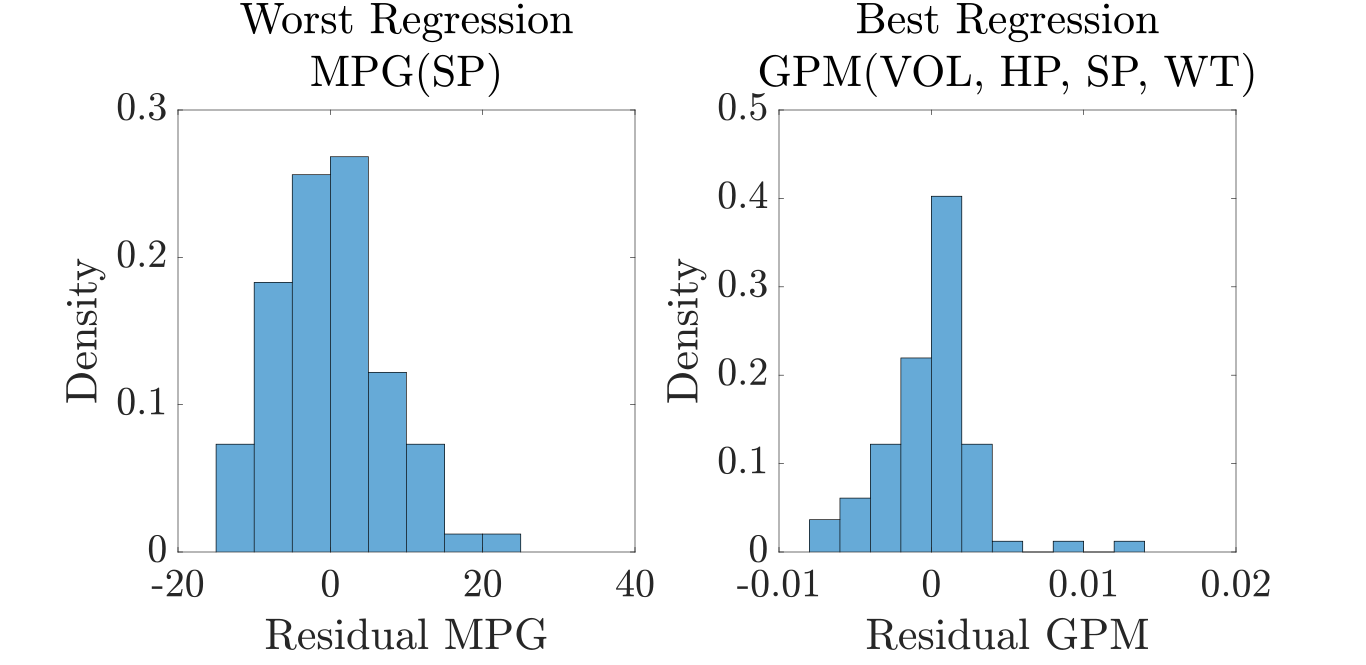
\includegraphics[width=0.45\textwidth]{Residuals}
    \caption{Residuals for best and worst $R^2_{adj}$ values.}
    \label{fig:Residuals}
\end{figure}

% References.
\printbibliography

\clearpage

\end{document}